%%%%%%%%%%%%%%%%%%%%%%%%%%%%%%%%%%%%%%%%%%%%%%%%%%%%%%%%%%%%%%%%%
% PARTE 3: EJERCICIOS PROPUESTOS Y SOLUCIONES
% Tema: Ecuaciones Trigonométricas
% 10 ejercicios con múltiples incisos + Soluciones completas
%%%%%%%%%%%%%%%%%%%%%%%%%%%%%%%%%%%%%%%%%%%%%%%%%%%%%%%%%%%%%%%%%

\section{Ejercicios Propuestos}

Ahora es tu turno de poner en práctica todo lo aprendido sobre ecuaciones trigonométricas. Te presento 10 ejercicios con diferentes niveles de dificultad. Intenta resolverlos por tu cuenta antes de ver las soluciones. ¡Recuerda que la práctica hace al maestro!

% EJERCICIOS BÁSICOS (1-3)

\begin{ejercicio}[title=Ejercicio 1: Ecuaciones básicas tipo f(x) = k]
Resuelve las siguientes ecuaciones trigonométricas en el intervalo $[0, 2\pi]$:
\begin{itemize}
    \item[a)] $\sin x = \frac{1}{2}$
    \item[b)] $\cos x = -\frac{\sqrt{3}}{2}$
    \item[c)] $\tan x = -1$
    \item[d)] $2\cos x - \sqrt{2} = 0$
\end{itemize}
\end{ejercicio}

\begin{ejercicio}[title=Ejercicio 2: Ecuaciones con transformaciones simples]
Encuentra todas las soluciones en el intervalo $[0°, 360°]$:
\begin{itemize}
    \item[a)] $\sin(x + 30°) = \frac{\sqrt{2}}{2}$
    \item[b)] $\cos(2x) = \frac{1}{2}$
    \item[c)] $\tan(x - 45°) = \sqrt{3}$
\end{itemize}
\end{ejercicio}

\begin{ejercicio}[title=Ejercicio 3: Ecuaciones con factores comunes]
Resuelve en el intervalo $[0, 2\pi]$:
\begin{itemize}
    \item[a)] $\sin x \cos x = 0$
    \item[b)] $2\sin x - 1 = 0$
    \item[c)] $(\cos x - 1)(\sin x + \frac{1}{2}) = 0$
\end{itemize}
\end{ejercicio}

% EJERCICIOS INTERMEDIOS (4-7)

\begin{ejercicio}[title=Ejercicio 4: Ecuaciones cuadráticas en una función]
Encuentra todas las soluciones en $[0, 2\pi]$:
\begin{itemize}
    \item[a)] $2\sin^2 x - \sin x - 1 = 0$
    \item[b)] $\cos^2 x - \cos x = 0$
    \item[c)] $\tan^2 x - 3 = 0$
    \item[d)] $4\cos^2 x - 3 = 0$
\end{itemize}
\end{ejercicio}

\begin{ejercicio}[title=Ejercicio 5: Ecuaciones con identidades trigonométricas]
Resuelve las siguientes ecuaciones en el intervalo $[0°, 360°]$:
\begin{itemize}
    \item[a)] $\sin^2 x + \cos x = 1$
    \item[b)] $2\cos^2 x - \sin x - 1 = 0$
    \item[c)] $\sec^2 x - 2\tan x = 0$
\end{itemize}
\end{ejercicio}

\begin{ejercicio}[title=Ejercicio 6: Ecuaciones con ángulos dobles]
Encuentra todas las soluciones en $[0, 2\pi]$:
\begin{itemize}
    \item[a)] $\sin(2x) = \sin x$
    \item[b)] $\cos(2x) = \cos x$
    \item[c)] $\sin(2x) = \frac{\sqrt{3}}{2}$
    \item[d)] $\cos(2x) + \sin x = 0$
\end{itemize}
\end{ejercicio}

\begin{ejercicio}[title=Ejercicio 7: Ecuaciones lineales en seno y coseno]
Resuelve en el intervalo $[0°, 360°]$:
\begin{itemize}
    \item[a)] $\sin x + \cos x = 1$
    \item[b)] $\sqrt{3}\sin x - \cos x = 1$
    \item[c)] $\sin x - \sqrt{3}\cos x = 2$
\end{itemize}
\end{ejercicio}

% EJERCICIOS AVANZADOS (8-10)

\begin{ejercicio}[title=Ejercicio 8: Ecuaciones con ángulos medios]
Encuentra todas las soluciones en $[0, 2\pi]$:
\begin{itemize}
    \item[a)] $2\sin\left(\frac{x}{2}\right) = 1$
    \item[b)] $\cos\left(\frac{x}{2}\right) = \cos x$
    \item[c)] $\tan\left(\frac{x}{2}\right) = \frac{\sin x}{1 + \cos x}$
\end{itemize}
\end{ejercicio}

\begin{ejercicio}[title=Ejercicio 9: Ecuaciones con múltiples funciones]
Resuelve en el intervalo $[0, 2\pi]$:
\begin{itemize}
    \item[a)] $\tan x + \cot x = 2$
    \item[b)] $\sin x + \cos x + \tan x = 1$
    \item[c)] $2\sin x \cos x = \cos x$
    \item[d)] $\sin^3 x + \sin x \cos^2 x = 0$
\end{itemize}
\end{ejercicio}

\begin{ejercicio}[title=Ejercicio 10: Ecuaciones con funciones inversas y aplicadas]
Resuelve las siguientes ecuaciones:
\begin{itemize}
    \item[a)] $2\arcsin(x) = \frac{\pi}{3}$ (encuentra el valor de $x$)
    \item[b)] $\sin x = \sin(2x)$ en $[0, 2\pi]$
    \item[c)] Una rueda de radio 10 metros gira. ¿En qué ángulos $\theta$ (medidos desde la horizontal) la altura del punto es exactamente 5 metros sobre el centro?
    \item[d)] La temperatura $T(t) = 20 + 10\sin\left(\frac{\pi t}{12}\right)$ modela la temperatura durante un día. ¿A qué horas $t$ (en $[0, 24]$) la temperatura es exactamente $25°C$?
\end{itemize}
\end{ejercicio}

\newpage

\section{Soluciones Detalladas}

Aquí están las soluciones completas de todos los ejercicios. Cada paso está explicado en detalle para que puedas entender el proceso de resolución.

% SOLUCIONES EJERCICIOS BÁSICOS (1-3)

\begin{solucion}[title=Solución Ejercicio 1]
\textbf{a) Resolver $\sin x = \frac{1}{2}$ en $[0, 2\pi]$}

\textbf{Paso 1:} Identificar el ángulo de referencia.
Sabemos que $\sin\left(\frac{\pi}{6}\right) = \frac{1}{2}$, entonces $\alpha = \frac{\pi}{6}$.

\textbf{Paso 2:} Determinar los cuadrantes donde el seno es positivo.
El seno es positivo en los cuadrantes I y II.

\textbf{Paso 3:} Encontrar las soluciones.
\begin{itemize}
    \item Cuadrante I: $x_1 = \frac{\pi}{6}$
    \item Cuadrante II: $x_2 = \pi - \frac{\pi}{6} = \frac{5\pi}{6}$
\end{itemize}

\textbf{Verificación:}
$\sin\left(\frac{\pi}{6}\right) = \frac{1}{2}$ ✓
$\sin\left(\frac{5\pi}{6}\right) = \frac{1}{2}$ ✓

\textbf{Respuesta:} $\boxed{x = \frac{\pi}{6}, \frac{5\pi}{6}}$

\vspace{0.3cm}

\textbf{b) Resolver $\cos x = -\frac{\sqrt{3}}{2}$ en $[0, 2\pi]$}

\textbf{Paso 1:} Ángulo de referencia.
Sabemos que $\cos\left(\frac{\pi}{6}\right) = \frac{\sqrt{3}}{2}$, entonces $\alpha = \frac{\pi}{6}$.

\textbf{Paso 2:} El coseno es negativo en los cuadrantes II y III.

\textbf{Paso 3:} Soluciones.
\begin{itemize}
    \item Cuadrante II: $x_1 = \pi - \frac{\pi}{6} = \frac{5\pi}{6}$
    \item Cuadrante III: $x_2 = \pi + \frac{\pi}{6} = \frac{7\pi}{6}$
\end{itemize}

\textbf{Respuesta:} $\boxed{x = \frac{5\pi}{6}, \frac{7\pi}{6}}$

\vspace{0.3cm}

\textbf{c) Resolver $\tan x = -1$ en $[0, 2\pi]$}

\textbf{Paso 1:} Ángulo de referencia.
Sabemos que $\tan\left(\frac{\pi}{4}\right) = 1$, entonces $\alpha = \frac{\pi}{4}$.

\textbf{Paso 2:} La tangente es negativa en los cuadrantes II y IV.

\textbf{Paso 3:} Soluciones.
\begin{itemize}
    \item Cuadrante II: $x_1 = \pi - \frac{\pi}{4} = \frac{3\pi}{4}$
    \item Cuadrante IV: $x_2 = 2\pi - \frac{\pi}{4} = \frac{7\pi}{4}$
\end{itemize}

\textbf{Respuesta:} $\boxed{x = \frac{3\pi}{4}, \frac{7\pi}{4}}$

\vspace{0.3cm}

\textbf{d) Resolver $2\cos x - \sqrt{2} = 0$ en $[0, 2\pi]$}

\textbf{Paso 1:} Despejar coseno.
\begin{align*}
2\cos x - \sqrt{2} &= 0 \\
2\cos x &= \sqrt{2} \\
\cos x &= \frac{\sqrt{2}}{2}
\end{align*}

\textbf{Paso 2:} Ángulo de referencia: $\alpha = \frac{\pi}{4}$.

\textbf{Paso 3:} El coseno es positivo en los cuadrantes I y IV.
\begin{itemize}
    \item Cuadrante I: $x_1 = \frac{\pi}{4}$
    \item Cuadrante IV: $x_2 = 2\pi - \frac{\pi}{4} = \frac{7\pi}{4}$
\end{itemize}

\textbf{Respuesta:} $\boxed{x = \frac{\pi}{4}, \frac{7\pi}{4}}$
\end{solucion}

\begin{solucion}[title=Solución Ejercicio 2]
\textbf{a) Resolver $\sin(x + 30°) = \frac{\sqrt{2}}{2}$ en $[0°, 360°]$}

\textbf{Paso 1:} Sea $u = x + 30°$, entonces $\sin u = \frac{\sqrt{2}}{2}$.

\textbf{Paso 2:} Resolver para $u$.
$\sin u = \frac{\sqrt{2}}{2}$ cuando $u = 45°$ o $u = 135°$ (más múltiplos de $360°$).

\textbf{Paso 3:} Como $u = x + 30°$:
\begin{align*}
x + 30° &= 45° \Rightarrow x = 15° \\
x + 30° &= 135° \Rightarrow x = 105°
\end{align*}

También consideramos el siguiente período:
\begin{align*}
x + 30° &= 45° + 360° = 405° \Rightarrow x = 375°
\end{align*}

Pero $375° > 360°$, así que no está en nuestro intervalo.

\textbf{Respuesta:} $\boxed{x = 15°, 105°}$

\vspace{0.3cm}

\textbf{b) Resolver $\cos(2x) = \frac{1}{2}$ en $[0°, 360°]$}

\textbf{Paso 1:} Sea $u = 2x$, entonces $\cos u = \frac{1}{2}$.

\textbf{Paso 2:} $\cos u = \frac{1}{2}$ cuando $u = 60°$ o $u = 300°$ (más múltiplos de $360°$).

\textbf{Paso 3:} Como $u = 2x$ y $x \in [0°, 360°]$, entonces $u \in [0°, 720°]$.

Las soluciones para $u$ son:
$u = 60°, 300°, 420°, 660°$

\textbf{Paso 4:} Despejar $x$:
\begin{align*}
2x = 60° &\Rightarrow x = 30° \\
2x = 300° &\Rightarrow x = 150° \\
2x = 420° &\Rightarrow x = 210° \\
2x = 660° &\Rightarrow x = 330°
\end{align*}

\textbf{Respuesta:} $\boxed{x = 30°, 150°, 210°, 330°}$

\vspace{0.3cm}

\textbf{c) Resolver $\tan(x - 45°) = \sqrt{3}$ en $[0°, 360°]$}

\textbf{Paso 1:} Sea $u = x - 45°$, entonces $\tan u = \sqrt{3}$.

\textbf{Paso 2:} $\tan u = \sqrt{3}$ cuando $u = 60°$ (más múltiplos de $180°$).

\textbf{Paso 3:} Las soluciones para $u$ son:
$u = 60°, 240°$ (en un período de $360°$)

\textbf{Paso 4:} Despejar $x$:
\begin{align*}
x - 45° = 60° &\Rightarrow x = 105° \\
x - 45° = 240° &\Rightarrow x = 285°
\end{align*}

\textbf{Respuesta:} $\boxed{x = 105°, 285°}$
\end{solucion}

\begin{solucion}[title=Solución Ejercicio 3]
\textbf{a) Resolver $\sin x \cos x = 0$ en $[0, 2\pi]$}

Un producto es cero si al menos uno de los factores es cero.

\textbf{Caso 1:} $\sin x = 0$
Esto ocurre cuando $x = 0, \pi, 2\pi$

\textbf{Caso 2:} $\cos x = 0$
Esto ocurre cuando $x = \frac{\pi}{2}, \frac{3\pi}{2}$

\textbf{Respuesta:} $\boxed{x = 0, \frac{\pi}{2}, \pi, \frac{3\pi}{2}, 2\pi}$

\vspace{0.3cm}

\textbf{b) Resolver $2\sin x - 1 = 0$ en $[0, 2\pi]$}

\begin{align*}
2\sin x - 1 &= 0 \\
\sin x &= \frac{1}{2}
\end{align*}

El seno es $\frac{1}{2}$ en los cuadrantes I y II:
\begin{itemize}
    \item $x = \frac{\pi}{6}$
    \item $x = \pi - \frac{\pi}{6} = \frac{5\pi}{6}$
\end{itemize}

\textbf{Respuesta:} $\boxed{x = \frac{\pi}{6}, \frac{5\pi}{6}}$

\vspace{0.3cm}

\textbf{c) Resolver $(\cos x - 1)(\sin x + \frac{1}{2}) = 0$ en $[0, 2\pi]$}

\textbf{Caso 1:} $\cos x - 1 = 0$
\begin{align*}
\cos x &= 1 \\
x &= 0, 2\pi
\end{align*}

\textbf{Caso 2:} $\sin x + \frac{1}{2} = 0$
\begin{align*}
\sin x &= -\frac{1}{2}
\end{align*}

El seno es $-\frac{1}{2}$ en los cuadrantes III y IV:
\begin{itemize}
    \item Cuadrante III: $x = \pi + \frac{\pi}{6} = \frac{7\pi}{6}$
    \item Cuadrante IV: $x = 2\pi - \frac{\pi}{6} = \frac{11\pi}{6}$
\end{itemize}

\textbf{Respuesta:} $\boxed{x = 0, \frac{7\pi}{6}, \frac{11\pi}{6}, 2\pi}$
\end{solucion}

% SOLUCIONES EJERCICIOS INTERMEDIOS (4-7)

\begin{solucion}[title=Solución Ejercicio 4]
\textbf{a) Resolver $2\sin^2 x - \sin x - 1 = 0$ en $[0, 2\pi]$}

Esta es una ecuación cuadrática en $\sin x$. Sea $u = \sin x$:
\begin{align*}
2u^2 - u - 1 &= 0
\end{align*}

Factorizando: $(2u + 1)(u - 1) = 0$

Por lo tanto: $u = -\frac{1}{2}$ o $u = 1$

\textbf{Caso 1:} $\sin x = -\frac{1}{2}$
\begin{itemize}
    \item Cuadrante III: $x = \pi + \frac{\pi}{6} = \frac{7\pi}{6}$
    \item Cuadrante IV: $x = 2\pi - \frac{\pi}{6} = \frac{11\pi}{6}$
\end{itemize}

\textbf{Caso 2:} $\sin x = 1$
\begin{itemize}
    \item $x = \frac{\pi}{2}$
\end{itemize}

\textbf{Respuesta:} $\boxed{x = \frac{\pi}{2}, \frac{7\pi}{6}, \frac{11\pi}{6}}$

\vspace{0.3cm}

\textbf{b) Resolver $\cos^2 x - \cos x = 0$ en $[0, 2\pi]$}

Factorizando:
\begin{align*}
\cos x(\cos x - 1) &= 0
\end{align*}

\textbf{Caso 1:} $\cos x = 0$
$x = \frac{\pi}{2}, \frac{3\pi}{2}$

\textbf{Caso 2:} $\cos x = 1$
$x = 0, 2\pi$

\textbf{Respuesta:} $\boxed{x = 0, \frac{\pi}{2}, \frac{3\pi}{2}, 2\pi}$

\vspace{0.3cm}

\textbf{c) Resolver $\tan^2 x - 3 = 0$ en $[0, 2\pi]$}

\begin{align*}
\tan^2 x &= 3 \\
\tan x &= \pm\sqrt{3}
\end{align*}

\textbf{Caso 1:} $\tan x = \sqrt{3}$
\begin{itemize}
    \item Cuadrante I: $x = \frac{\pi}{3}$
    \item Cuadrante III: $x = \pi + \frac{\pi}{3} = \frac{4\pi}{3}$
\end{itemize}

\textbf{Caso 2:} $\tan x = -\sqrt{3}$
\begin{itemize}
    \item Cuadrante II: $x = \pi - \frac{\pi}{3} = \frac{2\pi}{3}$
    \item Cuadrante IV: $x = 2\pi - \frac{\pi}{3} = \frac{5\pi}{3}$
\end{itemize}

\textbf{Respuesta:} $\boxed{x = \frac{\pi}{3}, \frac{2\pi}{3}, \frac{4\pi}{3}, \frac{5\pi}{3}}$

\vspace{0.3cm}

\textbf{d) Resolver $4\cos^2 x - 3 = 0$ en $[0, 2\pi]$}

\begin{align*}
4\cos^2 x &= 3 \\
\cos^2 x &= \frac{3}{4} \\
\cos x &= \pm\frac{\sqrt{3}}{2}
\end{align*}

\textbf{Caso 1:} $\cos x = \frac{\sqrt{3}}{2}$
\begin{itemize}
    \item Cuadrante I: $x = \frac{\pi}{6}$
    \item Cuadrante IV: $x = 2\pi - \frac{\pi}{6} = \frac{11\pi}{6}$
\end{itemize}

\textbf{Caso 2:} $\cos x = -\frac{\sqrt{3}}{2}$
\begin{itemize}
    \item Cuadrante II: $x = \pi - \frac{\pi}{6} = \frac{5\pi}{6}$
    \item Cuadrante III: $x = \pi + \frac{\pi}{6} = \frac{7\pi}{6}$
\end{itemize}

\textbf{Respuesta:} $\boxed{x = \frac{\pi}{6}, \frac{5\pi}{6}, \frac{7\pi}{6}, \frac{11\pi}{6}}$
\end{solucion}

\begin{solucion}[title=Solución Ejercicio 5]
\textbf{a) Resolver $\sin^2 x + \cos x = 1$ en $[0°, 360°]$}

Usando la identidad $\sin^2 x = 1 - \cos^2 x$:
\begin{align*}
1 - \cos^2 x + \cos x &= 1 \\
-\cos^2 x + \cos x &= 0 \\
\cos x(1 - \cos x) &= 0
\end{align*}

\textbf{Caso 1:} $\cos x = 0$
$x = 90°, 270°$

\textbf{Caso 2:} $\cos x = 1$
$x = 0°, 360°$

\textbf{Respuesta:} $\boxed{x = 0°, 90°, 270°, 360°}$

\vspace{0.3cm}

\textbf{b) Resolver $2\cos^2 x - \sin x - 1 = 0$ en $[0°, 360°]$}

Usando $\cos^2 x = 1 - \sin^2 x$:
\begin{align*}
2(1 - \sin^2 x) - \sin x - 1 &= 0 \\
2 - 2\sin^2 x - \sin x - 1 &= 0 \\
-2\sin^2 x - \sin x + 1 &= 0 \\
2\sin^2 x + \sin x - 1 &= 0
\end{align*}

Usando la fórmula cuadrática con $u = \sin x$:
\begin{align*}
u &= \frac{-1 \pm \sqrt{1 + 8}}{4} = \frac{-1 \pm 3}{4}
\end{align*}

Por lo tanto: $u = \frac{1}{2}$ o $u = -1$

\textbf{Caso 1:} $\sin x = \frac{1}{2}$
$x = 30°, 150°$

\textbf{Caso 2:} $\sin x = -1$
$x = 270°$

\textbf{Respuesta:} $\boxed{x = 30°, 150°, 270°}$

\vspace{0.3cm}

\textbf{c) Resolver $\sec^2 x - 2\tan x = 0$ en $[0°, 360°]$}

Usando la identidad $\sec^2 x = 1 + \tan^2 x$:
\begin{align*}
1 + \tan^2 x - 2\tan x &= 0 \\
\tan^2 x - 2\tan x + 1 &= 0 \\
(\tan x - 1)^2 &= 0 \\
\tan x &= 1
\end{align*}

La tangente es 1 cuando:
$x = 45°, 225°$

\textbf{Respuesta:} $\boxed{x = 45°, 225°}$
\end{solucion}

\begin{solucion}[title=Solución Ejercicio 6]
\textbf{a) Resolver $\sin(2x) = \sin x$ en $[0, 2\pi]$}

Usando la identidad $\sin(2x) = 2\sin x \cos x$:
\begin{align*}
2\sin x \cos x &= \sin x \\
2\sin x \cos x - \sin x &= 0 \\
\sin x(2\cos x - 1) &= 0
\end{align*}

\textbf{Caso 1:} $\sin x = 0$
$x = 0, \pi, 2\pi$

\textbf{Caso 2:} $\cos x = \frac{1}{2}$
$x = \frac{\pi}{3}, \frac{5\pi}{3}$

\textbf{Respuesta:} $\boxed{x = 0, \frac{\pi}{3}, \pi, \frac{5\pi}{3}, 2\pi}$

\vspace{0.3cm}

\textbf{b) Resolver $\cos(2x) = \cos x$ en $[0, 2\pi]$}

Usando $\cos(2x) = 2\cos^2 x - 1$:
\begin{align*}
2\cos^2 x - 1 &= \cos x \\
2\cos^2 x - \cos x - 1 &= 0
\end{align*}

Factorizando: $(2\cos x + 1)(\cos x - 1) = 0$

\textbf{Caso 1:} $\cos x = -\frac{1}{2}$
$x = \frac{2\pi}{3}, \frac{4\pi}{3}$

\textbf{Caso 2:} $\cos x = 1$
$x = 0, 2\pi$

\textbf{Respuesta:} $\boxed{x = 0, \frac{2\pi}{3}, \frac{4\pi}{3}, 2\pi}$

\vspace{0.3cm}

\textbf{c) Resolver $\sin(2x) = \frac{\sqrt{3}}{2}$ en $[0, 2\pi]$}

Sea $u = 2x$, entonces $\sin u = \frac{\sqrt{3}}{2}$.

Como $x \in [0, 2\pi]$, entonces $u \in [0, 4\pi]$.

$\sin u = \frac{\sqrt{3}}{2}$ cuando:
\begin{align*}
u &= \frac{\pi}{3}, \frac{2\pi}{3}, \frac{\pi}{3} + 2\pi, \frac{2\pi}{3} + 2\pi \\
u &= \frac{\pi}{3}, \frac{2\pi}{3}, \frac{7\pi}{3}, \frac{8\pi}{3}
\end{align*}

Despejando $x = \frac{u}{2}$:
\begin{align*}
x &= \frac{\pi}{6}, \frac{\pi}{3}, \frac{7\pi}{6}, \frac{4\pi}{3}
\end{align*}

\textbf{Respuesta:} $\boxed{x = \frac{\pi}{6}, \frac{\pi}{3}, \frac{7\pi}{6}, \frac{4\pi}{3}}$

\vspace{0.3cm}

\textbf{d) Resolver $\cos(2x) + \sin x = 0$ en $[0, 2\pi]$}

Usando $\cos(2x) = 1 - 2\sin^2 x$:
\begin{align*}
1 - 2\sin^2 x + \sin x &= 0 \\
2\sin^2 x - \sin x - 1 &= 0
\end{align*}

Factorizando: $(2\sin x + 1)(\sin x - 1) = 0$

\textbf{Caso 1:} $\sin x = -\frac{1}{2}$
$x = \frac{7\pi}{6}, \frac{11\pi}{6}$

\textbf{Caso 2:} $\sin x = 1$
$x = \frac{\pi}{2}$

\textbf{Respuesta:} $\boxed{x = \frac{\pi}{2}, \frac{7\pi}{6}, \frac{11\pi}{6}}$
\end{solucion}

\begin{solucion}[title=Solución Ejercicio 7]
\textbf{a) Resolver $\sin x + \cos x = 1$ en $[0°, 360°]$}

\textbf{Método 1: Sustitución}

Elevando al cuadrado ambos lados:
\begin{align*}
(\sin x + \cos x)^2 &= 1 \\
\sin^2 x + 2\sin x \cos x + \cos^2 x &= 1 \\
1 + 2\sin x \cos x &= 1 \\
2\sin x \cos x &= 0 \\
\sin x \cos x &= 0
\end{align*}

Esto ocurre cuando $\sin x = 0$ o $\cos x = 0$.

Verificando en la ecuación original:
\begin{itemize}
    \item Si $\sin x = 0$ y $\cos x = 1$: $0 + 1 = 1$ ✓ → $x = 0°, 360°$
    \item Si $\sin x = 0$ y $\cos x = -1$: $0 + (-1) = -1 \neq 1$ ✗
    \item Si $\sin x = 1$ y $\cos x = 0$: $1 + 0 = 1$ ✓ → $x = 90°$
    \item Si $\sin x = -1$ y $\cos x = 0$: $-1 + 0 = -1 \neq 1$ ✗
\end{itemize}

\textbf{Respuesta:} $\boxed{x = 0°, 90°, 360°}$

\vspace{0.3cm}

\textbf{b) Resolver $\sqrt{3}\sin x - \cos x = 1$ en $[0°, 360°]$}

Dividiendo todo entre 2:
\begin{align*}
\frac{\sqrt{3}}{2}\sin x - \frac{1}{2}\cos x &= \frac{1}{2}
\end{align*}

Reconocemos que $\frac{\sqrt{3}}{2} = \cos 30°$ y $\frac{1}{2} = \sin 30°$:
\begin{align*}
\cos 30° \sin x - \sin 30° \cos x &= \frac{1}{2}
\end{align*}

Usando la identidad $\sin(A - B) = \sin A \cos B - \cos A \sin B$:
\begin{align*}
\sin(x - 30°) &= \frac{1}{2}
\end{align*}

Por lo tanto:
\begin{align*}
x - 30° &= 30° \text{ o } x - 30° = 150° \\
x &= 60° \text{ o } x = 180°
\end{align*}

\textbf{Verificación:}
\begin{itemize}
    \item $x = 60°$: $\sqrt{3} \cdot \frac{\sqrt{3}}{2} - \frac{1}{2} = \frac{3}{2} - \frac{1}{2} = 1$ ✓
    \item $x = 180°$: $\sqrt{3} \cdot 0 - (-1) = 1$ ✓
\end{itemize}

\textbf{Respuesta:} $\boxed{x = 60°, 180°}$

\vspace{0.3cm}

\textbf{c) Resolver $\sin x - \sqrt{3}\cos x = 2$ en $[0°, 360°]$}

Expresamos la ecuación en la forma $R\sin(x + \alpha) = 2$.

Donde $R = \sqrt{1^2 + (-\sqrt{3})^2} = \sqrt{1 + 3} = 2$

Y $\tan \alpha = \frac{-\sqrt{3}}{1} = -\sqrt{3}$, entonces $\alpha = -60°$

La ecuación se convierte en:
\begin{align*}
2\sin(x - 60°) &= 2 \\
\sin(x - 60°) &= 1
\end{align*}

Por lo tanto:
\begin{align*}
x - 60° &= 90° \\
x &= 150°
\end{align*}

\textbf{Verificación:}
$\sin 150° - \sqrt{3}\cos 150° = \frac{1}{2} - \sqrt{3} \cdot \left(-\frac{\sqrt{3}}{2}\right) = \frac{1}{2} + \frac{3}{2} = 2$ ✓

\textbf{Respuesta:} $\boxed{x = 150°}$
\end{solucion}

% SOLUCIONES EJERCICIOS AVANZADOS (8-10)

\begin{solucion}[title=Solución Ejercicio 8]
\textbf{a) Resolver $2\sin\left(\frac{x}{2}\right) = 1$ en $[0, 2\pi]$}

\begin{align*}
\sin\left(\frac{x}{2}\right) &= \frac{1}{2}
\end{align*}

Sea $u = \frac{x}{2}$. Como $x \in [0, 2\pi]$, entonces $u \in [0, \pi]$.

$\sin u = \frac{1}{2}$ cuando:
\begin{align*}
u &= \frac{\pi}{6} \text{ o } u = \frac{5\pi}{6}
\end{align*}

Pero $\frac{5\pi}{6} > \pi$ no está en nuestro rango para $u$, así que:
$u = \frac{\pi}{6}$ o $u = \pi - \frac{\pi}{6} = \frac{5\pi}{6}$

Despejando $x = 2u$:
\begin{align*}
x &= 2 \cdot \frac{\pi}{6} = \frac{\pi}{3} \\
x &= 2 \cdot \frac{5\pi}{6} = \frac{5\pi}{3}
\end{align*}

\textbf{Respuesta:} $\boxed{x = \frac{\pi}{3}, \frac{5\pi}{3}}$

\vspace{0.3cm}

\textbf{b) Resolver $\cos\left(\frac{x}{2}\right) = \cos x$ en $[0, 2\pi]$}

Usando la identidad $\cos x = 2\cos^2\left(\frac{x}{2}\right) - 1$:
\begin{align*}
\cos\left(\frac{x}{2}\right) &= 2\cos^2\left(\frac{x}{2}\right) - 1
\end{align*}

Sea $u = \cos\left(\frac{x}{2}\right)$:
\begin{align*}
u &= 2u^2 - 1 \\
2u^2 - u - 1 &= 0 \\
(2u + 1)(u - 1) &= 0
\end{align*}

Por lo tanto: $u = -\frac{1}{2}$ o $u = 1$

\textbf{Caso 1:} $\cos\left(\frac{x}{2}\right) = -\frac{1}{2}$

$\frac{x}{2} = \frac{2\pi}{3}$ o $\frac{x}{2} = \frac{4\pi}{3}$

$x = \frac{4\pi}{3}$ o $x = \frac{8\pi}{3}$

Como $\frac{8\pi}{3} > 2\pi$, solo $x = \frac{4\pi}{3}$ está en nuestro intervalo.

\textbf{Caso 2:} $\cos\left(\frac{x}{2}\right) = 1$

$\frac{x}{2} = 0$ o $\frac{x}{2} = 2\pi$

$x = 0$ (el valor $x = 4\pi$ está fuera del intervalo)

\textbf{Respuesta:} $\boxed{x = 0, \frac{4\pi}{3}}$

\vspace{0.3cm}

\textbf{c) Verificar la identidad $\tan\left(\frac{x}{2}\right) = \frac{\sin x}{1 + \cos x}$}

Esta es una identidad conocida. Vamos a verificarla:

Partiendo del lado derecho:
\begin{align*}
\frac{\sin x}{1 + \cos x} &= \frac{2\sin\left(\frac{x}{2}\right)\cos\left(\frac{x}{2}\right)}{1 + 2\cos^2\left(\frac{x}{2}\right) - 1} \\
&= \frac{2\sin\left(\frac{x}{2}\right)\cos\left(\frac{x}{2}\right)}{2\cos^2\left(\frac{x}{2}\right)} \\
&= \frac{\sin\left(\frac{x}{2}\right)}{\cos\left(\frac{x}{2}\right)} \\
&= \tan\left(\frac{x}{2}\right)
\end{align*}

La identidad es válida para todo $x$ donde ambos lados estén definidos.

\textbf{Respuesta:} La identidad es verdadera para todo $x \neq \pi + 2k\pi$ (donde $\cos x \neq -1$).
\end{solucion}

\begin{solucion}[title=Solución Ejercicio 9]
\textbf{a) Resolver $\tan x + \cot x = 2$ en $[0, 2\pi]$}

\begin{align*}
\tan x + \cot x &= 2 \\
\tan x + \frac{1}{\tan x} &= 2 \\
\frac{\tan^2 x + 1}{\tan x} &= 2 \\
\tan^2 x + 1 &= 2\tan x \\
\tan^2 x - 2\tan x + 1 &= 0 \\
(\tan x - 1)^2 &= 0 \\
\tan x &= 1
\end{align*}

La tangente es 1 cuando $x = \frac{\pi}{4}$ o $x = \frac{5\pi}{4}$.

\textbf{Respuesta:} $\boxed{x = \frac{\pi}{4}, \frac{5\pi}{4}}$

\vspace{0.3cm}

\textbf{b) Resolver $\sin x + \cos x + \tan x = 1$ en $[0, 2\pi]$}

Reescribiendo $\tan x = \frac{\sin x}{\cos x}$:
\begin{align*}
\sin x + \cos x + \frac{\sin x}{\cos x} &= 1 \\
\frac{\sin x \cos x + \cos^2 x + \sin x}{\cos x} &= 1 \\
\sin x \cos x + \cos^2 x + \sin x &= \cos x \\
\sin x(\cos x + 1) + \cos^2 x - \cos x &= 0 \\
\sin x(\cos x + 1) + \cos x(\cos x - 1) &= 0
\end{align*}

Esta ecuación es compleja. Probemos valores especiales:

Para $x = 0$: $\sin 0 + \cos 0 + \tan 0 = 0 + 1 + 0 = 1$ ✓

Para $x = \frac{\pi}{2}$: $\sin \frac{\pi}{2} + \cos \frac{\pi}{2} + \tan \frac{\pi}{2}$ no está definida.

Para $x = \pi$: $\sin \pi + \cos \pi + \tan \pi = 0 + (-1) + 0 = -1$ ✗

Para $x = 2\pi$: $\sin 2\pi + \cos 2\pi + \tan 2\pi = 0 + 1 + 0 = 1$ ✓

\textbf{Respuesta:} $\boxed{x = 0, 2\pi}$

\vspace{0.3cm}

\textbf{c) Resolver $2\sin x \cos x = \cos x$ en $[0, 2\pi]$}

\begin{align*}
2\sin x \cos x - \cos x &= 0 \\
\cos x(2\sin x - 1) &= 0
\end{align*}

\textbf{Caso 1:} $\cos x = 0$
$x = \frac{\pi}{2}, \frac{3\pi}{2}$

\textbf{Caso 2:} $\sin x = \frac{1}{2}$
$x = \frac{\pi}{6}, \frac{5\pi}{6}$

\textbf{Respuesta:} $\boxed{x = \frac{\pi}{6}, \frac{\pi}{2}, \frac{5\pi}{6}, \frac{3\pi}{2}}$

\vspace{0.3cm}

\textbf{d) Resolver $\sin^3 x + \sin x \cos^2 x = 0$ en $[0, 2\pi]$}

Factorizando:
\begin{align*}
\sin x(\sin^2 x + \cos^2 x) &= 0 \\
\sin x \cdot 1 &= 0 \\
\sin x &= 0
\end{align*}

Por lo tanto: $x = 0, \pi, 2\pi$

\textbf{Respuesta:} $\boxed{x = 0, \pi, 2\pi}$
\end{solucion}

\begin{solucion}[title=Solución Ejercicio 10]
\textbf{a) Resolver $2\arcsin(x) = \frac{\pi}{3}$}

\begin{align*}
\arcsin(x) &= \frac{\pi}{6} \\
x &= \sin\left(\frac{\pi}{6}\right) \\
x &= \frac{1}{2}
\end{align*}

\textbf{Verificación:} $2\arcsin\left(\frac{1}{2}\right) = 2 \cdot \frac{\pi}{6} = \frac{\pi}{3}$ ✓

\textbf{Respuesta:} $\boxed{x = \frac{1}{2}}$

\vspace{0.3cm}

\textbf{b) Resolver $\sin x = \sin(2x)$ en $[0, 2\pi]$}

Usando $\sin(2x) = 2\sin x \cos x$:
\begin{align*}
\sin x &= 2\sin x \cos x \\
\sin x - 2\sin x \cos x &= 0 \\
\sin x(1 - 2\cos x) &= 0
\end{align*}

\textbf{Caso 1:} $\sin x = 0$
$x = 0, \pi, 2\pi$

\textbf{Caso 2:} $\cos x = \frac{1}{2}$
$x = \frac{\pi}{3}, \frac{5\pi}{3}$

\textbf{Respuesta:} $\boxed{x = 0, \frac{\pi}{3}, \pi, \frac{5\pi}{3}, 2\pi}$

\vspace{0.3cm}

\textbf{c) Rueda de radio 10 metros, altura 5 metros sobre el centro}

La altura de un punto en la rueda está dada por:
$h(\theta) = 10\sin\theta$

Queremos $h = 5$:
\begin{align*}
10\sin\theta &= 5 \\
\sin\theta &= \frac{1}{2}
\end{align*}

En $[0, 2\pi]$:
$\theta = \frac{\pi}{6}$ (30°) o $\theta = \frac{5\pi}{6}$ (150°)

\textbf{Interpretación:} El punto está a 5 metros sobre el centro cuando el radio forma un ángulo de 30° o 150° con la horizontal.

\textbf{Respuesta:} $\boxed{\theta = 30° \text{ y } 150°}$

\begin{center}
\begin{tikzpicture}[scale=0.9]
    % Ejes
    \draw[-{Latex},thick] (-3.5,0) -- (3.5,0) node[right] {$x$};
    \draw[-{Latex},thick] (0,-3.5) -- (0,3.5) node[above] {$y$};

    % Círculo (rueda)
    \draw[thick,blue] (0,0) circle (3);

    % Línea horizontal a altura 5 (escalada)
    \draw[dashed,green,thick] (-3.5,1.5) -- (3.5,1.5) node[right] {$h = 5$};

    % Puntos donde h = 5
    \filldraw[red] (30:3) circle (0.1);
    \filldraw[red] (150:3) circle (0.1);

    % Radios
    \draw[red,thick] (0,0) -- (30:3) node[midway,below right] {$r=10$};
    \draw[red,thick] (0,0) -- (150:3);

    % Ángulos
    \draw[-{Latex},orange,thick] (1,0) arc (0:30:1) node[midway,right] {$30°$};
    \draw[-{Latex},orange,thick] (1,0) arc (0:150:1) node[midway,above] {$150°$};

    \node at (0,-4) {Posiciones donde la altura es 5 metros};
\end{tikzpicture}
\end{center}

\vspace{0.3cm}

\textbf{d) Temperatura $T(t) = 20 + 10\sin\left(\frac{\pi t}{12}\right) = 25°C$}

\begin{align*}
20 + 10\sin\left(\frac{\pi t}{12}\right) &= 25 \\
10\sin\left(\frac{\pi t}{12}\right) &= 5 \\
\sin\left(\frac{\pi t}{12}\right) &= \frac{1}{2}
\end{align*}

Sea $u = \frac{\pi t}{12}$. Como $t \in [0, 24]$, entonces $u \in [0, 2\pi]$.

$\sin u = \frac{1}{2}$ cuando:
$u = \frac{\pi}{6}$ o $u = \frac{5\pi}{6}$

Despejando $t$:
\begin{align*}
\frac{\pi t}{12} = \frac{\pi}{6} &\Rightarrow t = 2 \text{ horas} \\
\frac{\pi t}{12} = \frac{5\pi}{6} &\Rightarrow t = 10 \text{ horas}
\end{align*}

\textbf{Interpretación:} La temperatura es de 25°C a las 2:00 AM y a las 10:00 AM.

\textbf{Gráfica de la temperatura:}

\begin{center}
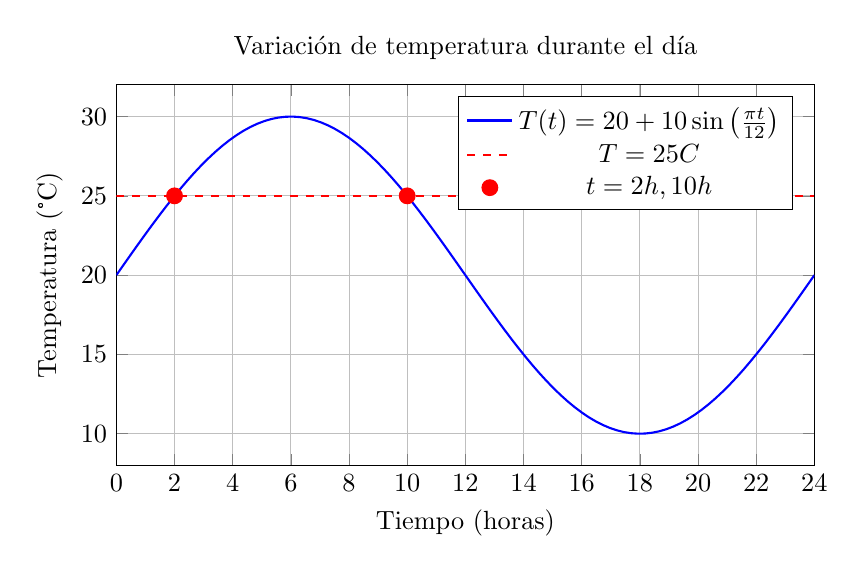
\begin{tikzpicture}[scale=0.95]
\begin{axis}[
    width=0.9\textwidth,
    height=0.55\textwidth,
    domain=0:24,
    samples=100,
    grid=major,
    xlabel={Tiempo (horas)},
    ylabel={Temperatura (°C)},
    title={Variación de temperatura durante el día},
    xmin=0, xmax=24,
    ymin=8, ymax=32,
    xtick={0,2,4,6,8,10,12,14,16,18,20,22,24},
    ytick={10,15,20,25,30},
    legend pos=north east,
]
    % Función de temperatura
    \addplot[blue,thick] {20 + 10*sin(pi*x/12 * 180/pi)};
    \addlegendentry{$T(t) = 20 + 10\sin\left(\frac{\pi t}{12}\right)$}

    % Línea horizontal en T = 25
    \addplot[red,dashed,thick] coordinates {(0,25) (24,25)};
    \addlegendentry{$T = 25°C$}

    % Puntos de intersección
    \addplot[only marks,mark=*,mark size=3pt,red] coordinates {(2,25) (10,25)};
    \addlegendentry{$t = 2h, 10h$}
\end{axis}
\end{tikzpicture}
\end{center}

\textbf{Respuesta:} $\boxed{t = 2 \text{ horas (2:00 AM) y } t = 10 \text{ horas (10:00 AM)}}$
\end{solucion}

\newpage

\section{Conclusión}

¡Felicitaciones! Has completado esta guía exhaustiva sobre ecuaciones trigonométricas. A lo largo de estos ejercicios has practicado:

\begin{itemize}
    \item \textbf{Ecuaciones básicas:} Tipo $f(x) = k$
    \item \textbf{Ecuaciones lineales:} Combinaciones de seno y coseno
    \item \textbf{Ecuaciones cuadráticas:} Usando sustitución y factorización
    \item \textbf{Ecuaciones con identidades:} Aplicando las identidades fundamentales
    \item \textbf{Ecuaciones con ángulos múltiples:} Dobles y medios
    \item \textbf{Aplicaciones prácticas:} Modelado de fenómenos reales
\end{itemize}

\subsection*{Consejos finales para resolver ecuaciones trigonométricas}

\begin{enumerate}
    \item \textbf{Identifica el tipo:} ¿Es lineal, cuadrática, o requiere identidades?
    \item \textbf{Simplifica primero:} Usa identidades para reducir a una sola función si es posible
    \item \textbf{Considera el dominio:} Siempre verifica que tus soluciones estén en el intervalo pedido
    \item \textbf{No olvides todos los casos:} Las funciones trigonométricas son periódicas
    \item \textbf{Verifica siempre:} Sustituye tus respuestas en la ecuación original
    \item \textbf{Dibuja cuando sea útil:} La circunferencia unitaria es tu mejor amiga
\end{enumerate}

\subsection*{Errores comunes a evitar}

\begin{itemize}
    \item Olvidar soluciones en otros cuadrantes
    \item No considerar el período completo
    \item Dividir por expresiones que podrían ser cero
    \item No verificar las soluciones en la ecuación original
    \item Confundir grados con radianes
\end{itemize}

Recuerda: La práctica constante es la clave para dominar las ecuaciones trigonométricas. ¡Sigue practicando y verás cómo cada vez te resultan más naturales!